\chapter{Métricas de Software}

\section{Processo de Medição de Software}

Segundo \citeonline{Fenton98}, medição é o mapeamento de relações empíricas em relações formais. Isto é, quantificação em símbolos com objetivo de caracterizar uma entidade por meio de seus atributos. Contrapondo-se com uma  definição operacional, a \citeonline{ISO:15939} define medição como conjunto de operações que visam por meio de um objeto determinar um valor a uma medida ou métrica. \footnote{A definição formal da \citeonline{ISO:15939} não utiliza o termo métrica, sendo que este é utilizado por abordagens mais antigas como GQM em \citeonline{Basili96b}, que é uma outra abordagem para medição, contudo compreende-se que o termo medida tem valor semântico equivalente ao de métrica no contexto do deste trabalho}. Alguns modelos de referência, como \citeonline{cmmi2010}, e até a própria \citeonline{ISO:15939} definem medição como uma ferramenta primordial para gerenciar as atividades do desenvolvimento de software e para avaliar a qualidade dos produtos e a capacidade de processos organizacionais. 


A \citeonline{ISO:15939} define um processo de medição com base em um modelo de
informação, que é mostrado na Figura \ref{informação}, afim de obter produtos de informação para cada necessidade de informação. Para isto, cada necessidade de informação, que é uma situação que requer conhecimento com intuito de  gerenciar objetivos, metas, riscos e problemas é mapeada em uma construção  mensurável que tem em sua origem um conceito mensurável,como por exemplo,  tamanho, qualidade, custo afim de mapear um atributo, que é uma característica  que permite distinguir qualitivativamente e/ou quantitativamente uma entidade, que pode ser um processo, projeto ou produto de software. Por fim  cada construção mensurável é mapeada em um ou mais produtos de informação que  levam uma ou mais métricas ou medidas, que podem ser classificadas sob  critérios apresentados na seção \ref{Classificação das Métricas de Software}.

\begin{figure}[h!]
\centering
	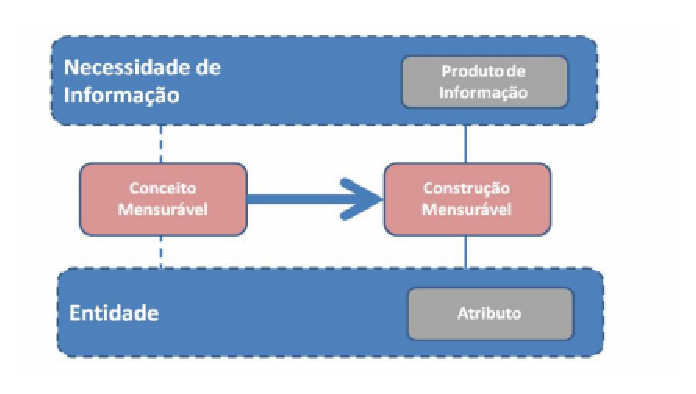
\includegraphics[keepaspectratio=true,scale=1]{figuras/mensuravel.eps}
	\caption{Modelo de Informação da ISO 15939 extraído de 
	\citeonline{manuela2011}}
	\label{informação}
\end{figure}
\FloatBarrier

O modelo de informação da \citeonline{ISO:15939} é utilizado para construir o 
propósito geral da medições e a identificação de medidas ou métricas que 
respondem as necessidades de informação. Em metodologias ágeis, como por exemplo, é possível construir um modelo de informação tal como na 
Tabela \ref{construção-ágil}.

	\begin{table}[!ht]
	\begin{center}
	 \begin{tabular}{|l|l|}
		\hline
		Entidade  & Código Fonte 
		\\ \hline
		Conceito Mensurável       & Qualidade      
		\\ \hline
		Construção Mensurável       & Qualidade do Código-Fonte      
		\\ \hline
		Atributos a ser medidos & Classes, Métodos e Pacotes   
		\\ \hline
		Produto de Informação   & Indicadores de Qualidade do Código-Fonte      
		\\ \hline
		\end{tabular}
		\caption{Modelo de Informação para metodologias ágeis com base na 
		\citeonline{ISO:15939}}
		\label{construção-ágil}
		\end{center}
		\end{table}		

%---------------------------------------------------------------------------------------------------------------------%

\section{Classificação das Métricas de Software}	
\label{Classificação das Métricas de Software}

As métricas de software possuem uma escala de medição, que é um conjunto 
ordenado de valores, contínuos ou discretos, ou uma série de categorias as 
quais entidade é mapeada \cite{ISO:15939}. As escalas podem ser:

\begin{easylist}[itemize]

& Nominal: A medição é categórica. Nesta escala, só é possível realização de 
comparações, sendo que a ordem não possui significado
\cite{ISO:15939} \cite{Fenton98} \cite{Meirelles2013}.

& Ordinal: A medição é baseada em ordenação, ou seja os valores possuem 
ordem, mas a distância entre eles não possui significado. Por exemplo, nível 
de experiência dos programadores \cite{ISO:15939} \cite{Fenton98} 
\cite{Meirelles2013}. 

& Intervalo: A medição é baseada em distâncias iguais definidas para as 
menores unidade. Por exemplo, o aumentar de 1º C de um termômetro. Nesta 
escala é possível realizar ordenação, soma e subtração. 
\cite{ISO:15939} \cite{Fenton98} 

& Racional: A medição é baseada em distâncias iguais definidas para as 
menores unidades, e neste caso é possível a ausência por meio do zero 
absoluto. Como por exemplo, a quantidade de linhas de código em uma classe. 
Nesta escala, é possível realizar ordenação, soma, subtração, 
multiplicação e divisão. \cite{ISO:15939} \cite{Fenton98} 

\end{easylist}
	
As métricas podem ser classificadas quanto a objeto da métrica, que 
divide as métricas de software em: \textit{métricas de processo} e 
\textit{métricas de produto} \cite{Mills:1999}. Ainda é possível, segundo a 
\citeonline{ISO:15939}, dividir as métricas quanto ao método de medição, 
podendo estas serem \textit{métricas objetivas}, que são baseadas em regras 
númericas e podem ter a coleta manual ou automática ou \textit{métricas 
subjetivas}, que envolvem o julgamento humano para consolidação do resultado. 

Segundo o modelo de qualidade da \citeonline{ISO25023}, que é mostrado na 
Figura \ref{modelodequalidade}, as métricas de produto podem ser subdivididas 
em três categorias: 

				
\begin{figure}[h!]
\centering
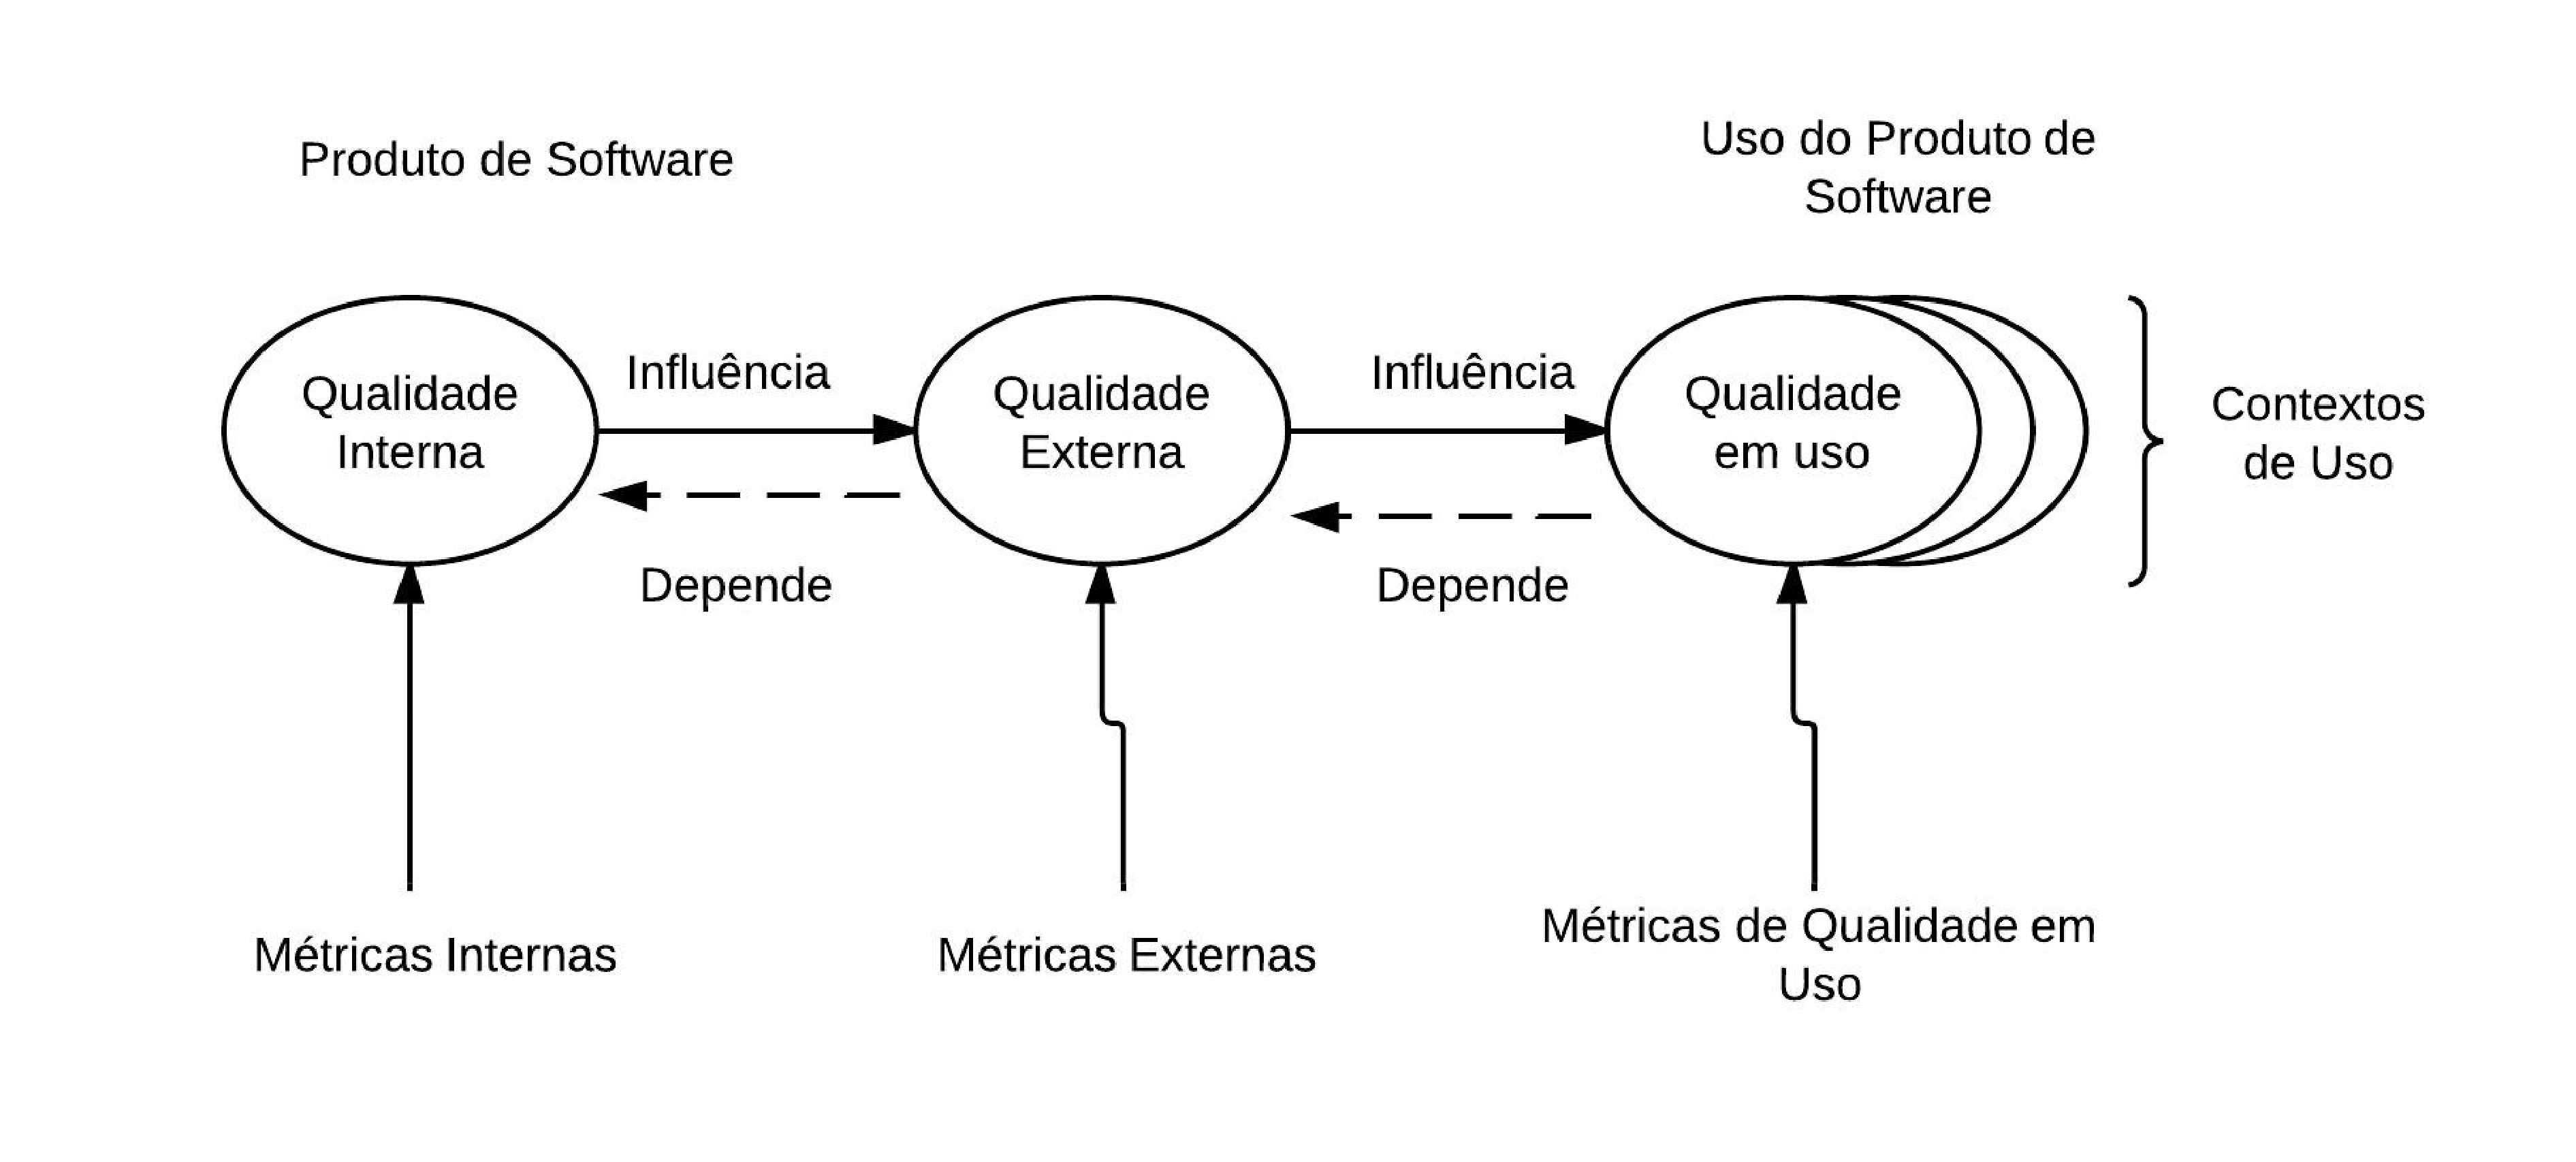
\includegraphics[keepaspectratio=false,scale=1]{figuras/modelodequalidade.eps}
\caption{Modelo de Qualidade do Produto da ISO 25023 adaptado de 
\citeonline{ISO25023}}
\label{modelodequalidade}
\end{figure}
\FloatBarrier
	
\begin{description}
%-----------------------------
		\item[Métricas Internas.] 
		São métricas que aferem a qualidade interna do software por meio da 
		avaliação de estruturas internas que compõem o software em estágio de 
		desenvolvimento. São conhecidas como métricas de código-fonte.

%-----------------------------			
		\item[Métricas Externas.]
		São métricas que capturam o comportamento do software. Exemplos de 
		atributos da qualidade externa: correção, usabilidade, eficiência e 
		robustez. Qualidade externa mede o comportamento do software. Estas só 
		podem ser aferidas por atividades de teste do desenvolvimento do 
		software em condições similares as que serão encontradas em ambientes de
		implantação.

%-----------------------------			
		\item[Métricas de Qualidade em Uso.]
		 São métricas que aferem se o software atende as necessidades do cliente
		 com eficiência, produtividade, segurança e satisfação em contextos 
		 específicos de uso. Estas só podem ser coletadas em ambientes reais, 
		 isto é, o ambiente de implantação.
			 
\end{description}
		
				

%---------------------------------------------------------------------------------------------------------------------%
\section {Métricas de Código-Fonte}
\label{Métricas de Código-Fonte}

Segundo a \textit{International Working Conference on Source Code Analysis and 
Manipulation} (SCAM), O código-fonte é qualquer especificação executável 
de um sistema de software. Por conseguinte, se inclui desde código de máquina, 
até linguagens de alto nível ou representações gráficas executáveis. 
\cite{harman2010source}. 


Portanto as métricas de código-fonte que são obtidas por meio da análise estática de código-fonte são obtidas por meio de especificações executáveis do software, isto é, trechos de código escritos em alguma linguagem de programação, são métricas objetivas e tem características como validade, simplicidade, objetividade, fácil obtenção e robustez \cite{Mills:1999}. \citeonline{Meirelles2013} realizou um levantamento sistemático na literatura das métricas de código-fonte. Estas foram categorizadas, nas seguintes categorias, apresentadas nas subseções a seguir. 


%--------------------------------------------
\subsection{Métrica de Tamanho e Complexidade}

\label{métricas tamanho e complexidade} 

O tamanho do código-fonte foi um dos primeiros conceitos mensuráveis do 
software, dado que o software poderia ocupar espaço tanto em forma de cartões 
perfurados quanto em forma de papel quando o código-fonte é impresso. 
A segunda lei de \citeonline{Lehman1980b} enuncia que a complexidade aumenta à 
medida que o software é evoluído, a menos que seja um trabalho de manutenção. 
Logo é perceptível que as métricas de complexidade estão diretamente ligadas as 
métricas de tamanho, sendo que a modificação em uma provavelmente impactará na 
outra. A seguir são apresentadas as principais métricas de tamanho e 
complexidade:


\begin{description}

	\item[LOC (\textit{Lines of Code})] \textbf{Número de Linhas de Código} 
	foi uma das primeiras métricas utilizadas para medir o tamanho de um 
	software. São contadas apenas as linhas executáveis, ou seja, são excluídas 
	linhas em branco e comentários. Para efetuar comparações entre sistemas 
	usando LOC, é necessário que ambos tenham sido feitos na mesma linguagem de 
	programação e que o estilo esteja normalizado \cite{Jones91}.
	
	\item[ACCM (\textit{Average Cyclomatic Complexity per Method})] \textbf{
	Média da Complexidade Ciclomática por Método} mede a complexidade do 
	métodos ou funções de um programa. Essa métrica pode ser representada 
	através de um grafo de fluxo de controle \cite{McCabe76}. O uso de 
	estruturas de controle, tais como, \textit{if, else, while} aumentam a 
	complexidade ciclomática de um de um método.

\end{description}




\subsection{Métricas de Orientação à Objetos}
\label{métrica objetos}

A evolução dos paradigmas de programação permitiu que as linguagens de 
programação, assumissem diversas características entre si. O paradigma 
funcional, por exemplo, enxerga o programa como uma sequência de funções que 
podem ser executadas em modo funcional. Já o paradigma orientado a objetos visa 
abstrair as unidades computacionais em Classes, que representam em grande 
parte do desenvolvimento, unidades reais do negócio, partindo destas abstrai-se instâncias 
computacionais, isto são, objetos propriamente ditos. A seguir são apresentadas 
as principais métricas de orientação à objetos:

\begin{description}

	\item[ACC (\textit{Afferent Connections per Class})] 
	\textbf{Conexões Aferentes por Classe} é número total de classes externas 
	de um pacote que dependem de classes de dentro desse pacote. Quando 
	calculada no nível da classe, essa medida também é conhecida como 
	\textit{Fan-in} da classe, medindo o número de classes das quais a classe é 
	derivada e, assim, valores elevados indicam uso excessivo de herança 
	múltipla \cite{McCabe94} \cite{Chidamber94}.
	
	
	%-----------------------------
	\item[RFC (\textit{Response For a Class})] \textbf{Respostas para uma 
	Classe} é número de métodos dentre todos os métodos que podem ser invocados 
	em resposta a uma mensagem enviada por um objeto de uma classe 
	\cite{Sharble93}.
	
	\item[LCOM4 (\textit{Lack of Cohesion in Methods})] \textbf{Falta de Coesão
	entre Métodos}. Originalmente proposto por \citeonline{Chidamber94} 
	como LCOM, contudo essa não teve uma grande aceitabilidade. Após críticas e 
	sugestões a métrica revisada por \citeonline{LCOM4}, que propôs a LCOM4. 
	Para calcular LCOM4 de um módulo, é necessário construir um gráfico 
	não-orientado em que os nós são os métodos e atributos de uma classe. Para
	cada método, deve haver uma aresta entre ele e um outro método ou variável 
	que ele usa. O valor da LCOM4 é o número de componentes fracamente 
	conectados nesse gráfico. 

	
	%-----------------------------
	\item[NOM (\textit{Number of Methods})] \textbf{Número de Métodos} é usado 
	para medir o tamanho das classes em termos das suas operações 
	implementadas. Essa métrica é usada para ajudar a identificar o 
	potencial de reúso de uma classe. Em geral, as classes com um grande 
	número de métodos são mais difíceis de serem reutilizadas, pois elas 
	são propensas a serem menos coesa \cite{Lorenz94}.
	

	%-----------------------------
	\item [DIT (\textit{Depth of Inheritance Tree})] \textbf{Profundidade da 
	Árvore de Herança} é o número de superclasses ou classes ancestrais da 
	classe sendo analisada. São contabilizadas apenas as superclasses do 
	sistema, ou seja, as classes de bibliotecas não são contabilizadas. 
	Nos casos onde herança múltipla é permitida, considera-se o maior 
	caminho da classe até uma das raízes da hierarquia. Quanto maior for o 
	valor DIT, maior é o número de atributos e métodos herdados, e portanto 
	maior é a complexidade \cite{Shih97}.
	
	\item[NOC (\textit{Number of Children})] \textbf{Número de Filhos} é o 
	número subclasses ou classes filhas que herdam da classe analisada 
	\cite{Rosenberg97}. Deve se ter cautela ao modificar classes com muitos 
	filhos, pois uma simples modificação de assinatura de um método, pode criar
	uma mudança em muitas classes.
	

\end{description}
	
\subsection{Intervalos da Métricas}
\label{Intervalos das Métricas}
Em sua tese \citeonline{Meirelles2013} analisou as métricas do código-fonte de 
38 projetos de software livre, em um total de 344.872 classes das aplicações 
mais bem sucedidas (\textit{Chrome, Firefox, OpenJDK, VLC e entre outros}) e 
percebeu que há certos valores que são frequentemente encontrados quando se 
analisa o código-fonte de aplicações que utilizam a mesma linguagem de 
programação. \citeonline{Meirelles2013}, após uma análise estatística com o 75º percentil dos valores obtidos para cada métrica de código-fonte, classificou estes 
intervalos, em \textit{muito frequente, frequente, pouco frequente e não 
frequente}. 

Visando o melhor entendimento das métricas, resolveu-se renomear tal como a 
Tabela \ref{nomes}. Posteriormente, é apresentada a Tabela \ref{metrics}, 
decorrente do estudo de \citeonline{Meirelles2013}, com os intervalos 
encontrados para C++ e Java.

	\begin{table}[!ht]
	\begin{center}
	 \begin{tabular}{|l|l|}
		\hline
		Intervalo de Frequência & Indicador Qualitativo \\ \hline
		Muito Frequente & Excelente \\ \hline
		Frequente       & Bom       \\ \hline
		Pouco Frequente & Regular   \\ \hline
		Não Frequente   & Ruim      \\ \hline
		\end{tabular}
		\caption{Nome dos Intervalos de Frequência}
		\label{nomes}
		\end{center}
		\end{table}
		
\FloatBarrier
	
	\begin{table}[!ht]
	\begin{center}
	\begin{tabular}{ |l|l|l|l| }
		\hline
		Métrica & Indicador & Java & C++ \\ \hline
		%-------------------------------
		\multirow{4}{*}{LOC} 
		 & Excelente & [de 0 a 33] & [de 0 a 31] \\
		 & Bom & [de 34 a 87] & [de 32 a 84] \\
		 & Regular & [de 88 a 200] & [de 85 a 207] \\
		 & Ruim & [acima de 200] & [acima de 207] \\ \hline
		 %---------------------------------
		 
		 %-------------------------------
		\multirow{4}{*}{ACCM} 
		 & Excelente & [de 0 a 2,8] & [de 0 a 2,0] \\
		 & Bom & [de 2,9 a 4,4] & [de 2,1 a 4,0] \\
		 & Regular & [de 4,5 a 6,0] & [de 4,1 a 6,0] \\
		 & Ruim & [acima de 6] & [acima de 6] \\ \hline
		 %---------------------------------
		 
		 
		%-------------------------------
		\multirow{4}{*}{ACC} 
		 & Excelente & [de 0 a 1] & [de 0 a 2,0] \\
		 & Bom & [de 1,1 a 5] & [de 2,1 a 7,0] \\
		 & Regular & [de 5,1 a 12] & [de 7,1 a 15] \\
		 & Ruim & [acima de 12] & [acima de 15] \\ \hline
		 %---------------------------------
	
		 
		%-------------------------------
		\multirow{4}{*}{RFC} 
		 & Excelente & [de 0 a 9] & [de 0 a 29] \\
		 & Bom & [de 10 a 26] & [de 30 a 64] \\
		 & Regular & [de 27 a 59] & [de 65 a 102] \\
		 & Ruim & [acima de 59] & [acima de 102] \\ \hline
		 %---------------------------------
		 
		 %-------------------------------
		\multirow{4}{*}{LCOM4} 
		 & Excelente & [de 0 a 3] & [de 0 a 5] \\
		 & Bom & [de 4 a 7] & [de 6 a 10] \\
		 & Regular & [de 8 a 12] & [de 11 a 14] \\
		 & Ruim & [acima de 12] & [acima de 14] \\ \hline
		 %---------------------------------
		 
		 %-------------------------------
		\multirow{4}{*}{NOM} 
		 & Excelente & [de 0 a 8] & [de 0 a 10] \\
		 & Bom & [de 9 a 17] & [de 11 a 17] \\
		 & Regular & [de 18 a 27] & [de 18 a 26] \\
		 & Ruim & [acima de 27] & [acima de 26] \\ \hline
		 %---------------------------------
		 
		 %-------------------------------
		\multirow{4}{*}{DIT} 
		 & Excelente & [de 0 a 2] & [de 0 a 1] \\
		 & Bom & [de 3 a 4] & [de 2 a 3] \\
		 & Regular & [de 5 a 6] & [de 3 a 4] \\
		 & Ruim & [acima de 6] & [acima de 4] \\ \hline
		 %---------------------------------
		
		%-------------------------------
		\multirow{4}{*}{NOC} 
		 & Excelente & [de 0 a 1] & [0] \\
		 & Bom & [de 1 a 2] & [1] \\
		 & Regular & [de 2 a 3] & [de 1 a 2] \\
		 & Ruim & [acima de 3] & [acima de 2] \\ \hline
		 %---------------------------------
		 
	\end{tabular}
	\caption{Intervalos das Métricas para Java e C++}
	\label{metrics}
	\end{center}
	\end{table}

\FloatBarrier
	
Os intervalos, que foram apresentados na Tabela \ref{metrics} serão utilizados
como indicadores de qualidade de código-fonte, de modo a simplificar a 
interpretação da qualidade do código-fonte no componente de visualização de dados, do ambiente de \textit{Data Warehousing}, a ser apresentado a seguir.